\chapter{Model Description}
\label{ch:chapter4}
As mentioned in Chapter 1, I am using a model of the \Gls{msbr}
\cite{robertson_conceptual_1971} to verify my \OpenMC implementation in
\SaltProc.

I picked the \Gls{msbr} because\ldots 

The \Gls{msbr} design is the result of a design study of a single-fluid
\Gls{msr} following the success of the \Gls{msre}
\cite{haubenreich_experience_1970}\cite{rosenthal_molten-salt_1970}.
I will only describe the following reactor systems that are relevant to
my validation study\footnote{A complete description of the entire \Gls{msbr}
system can be found in \cite{robertson_conceptual_1971}}: the fuel salt, the
reactor core, and the salt reprocessing system.

\begin{figure}[htpb] 
    \label{fig:msbr-overview}
    \centering
    \subfloat[][]{
        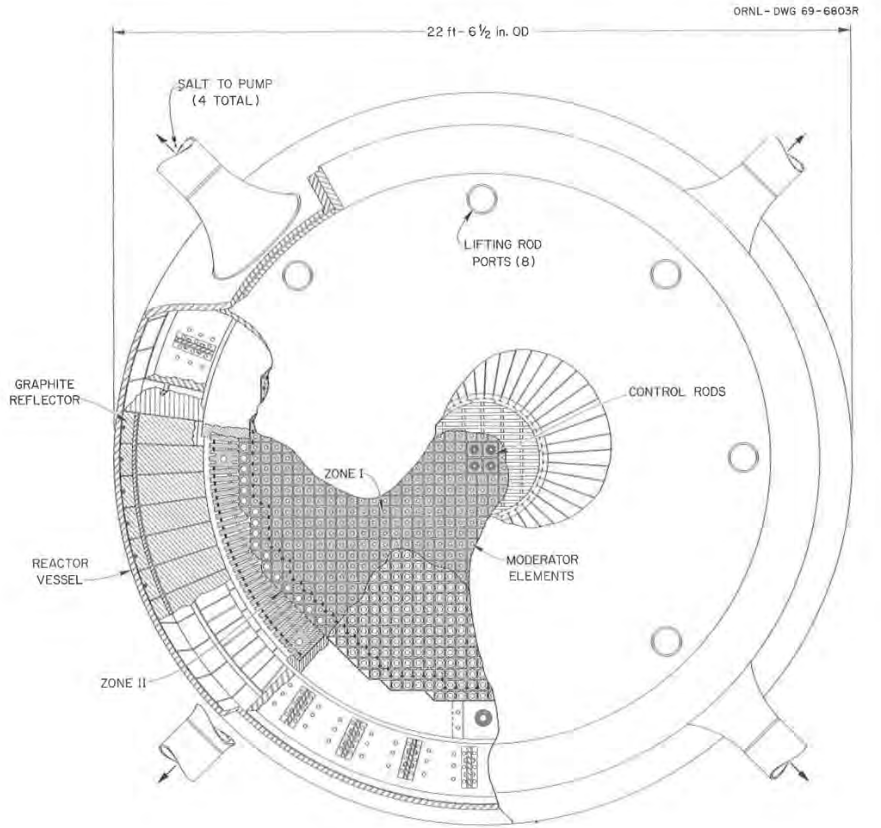
\includegraphics[width=0.5\linewidth]{figs/ch4/msbr_full_xy_ref.png}
        \label{fig:msbr_ref_xy}
    }
    \subfloat[][]{
        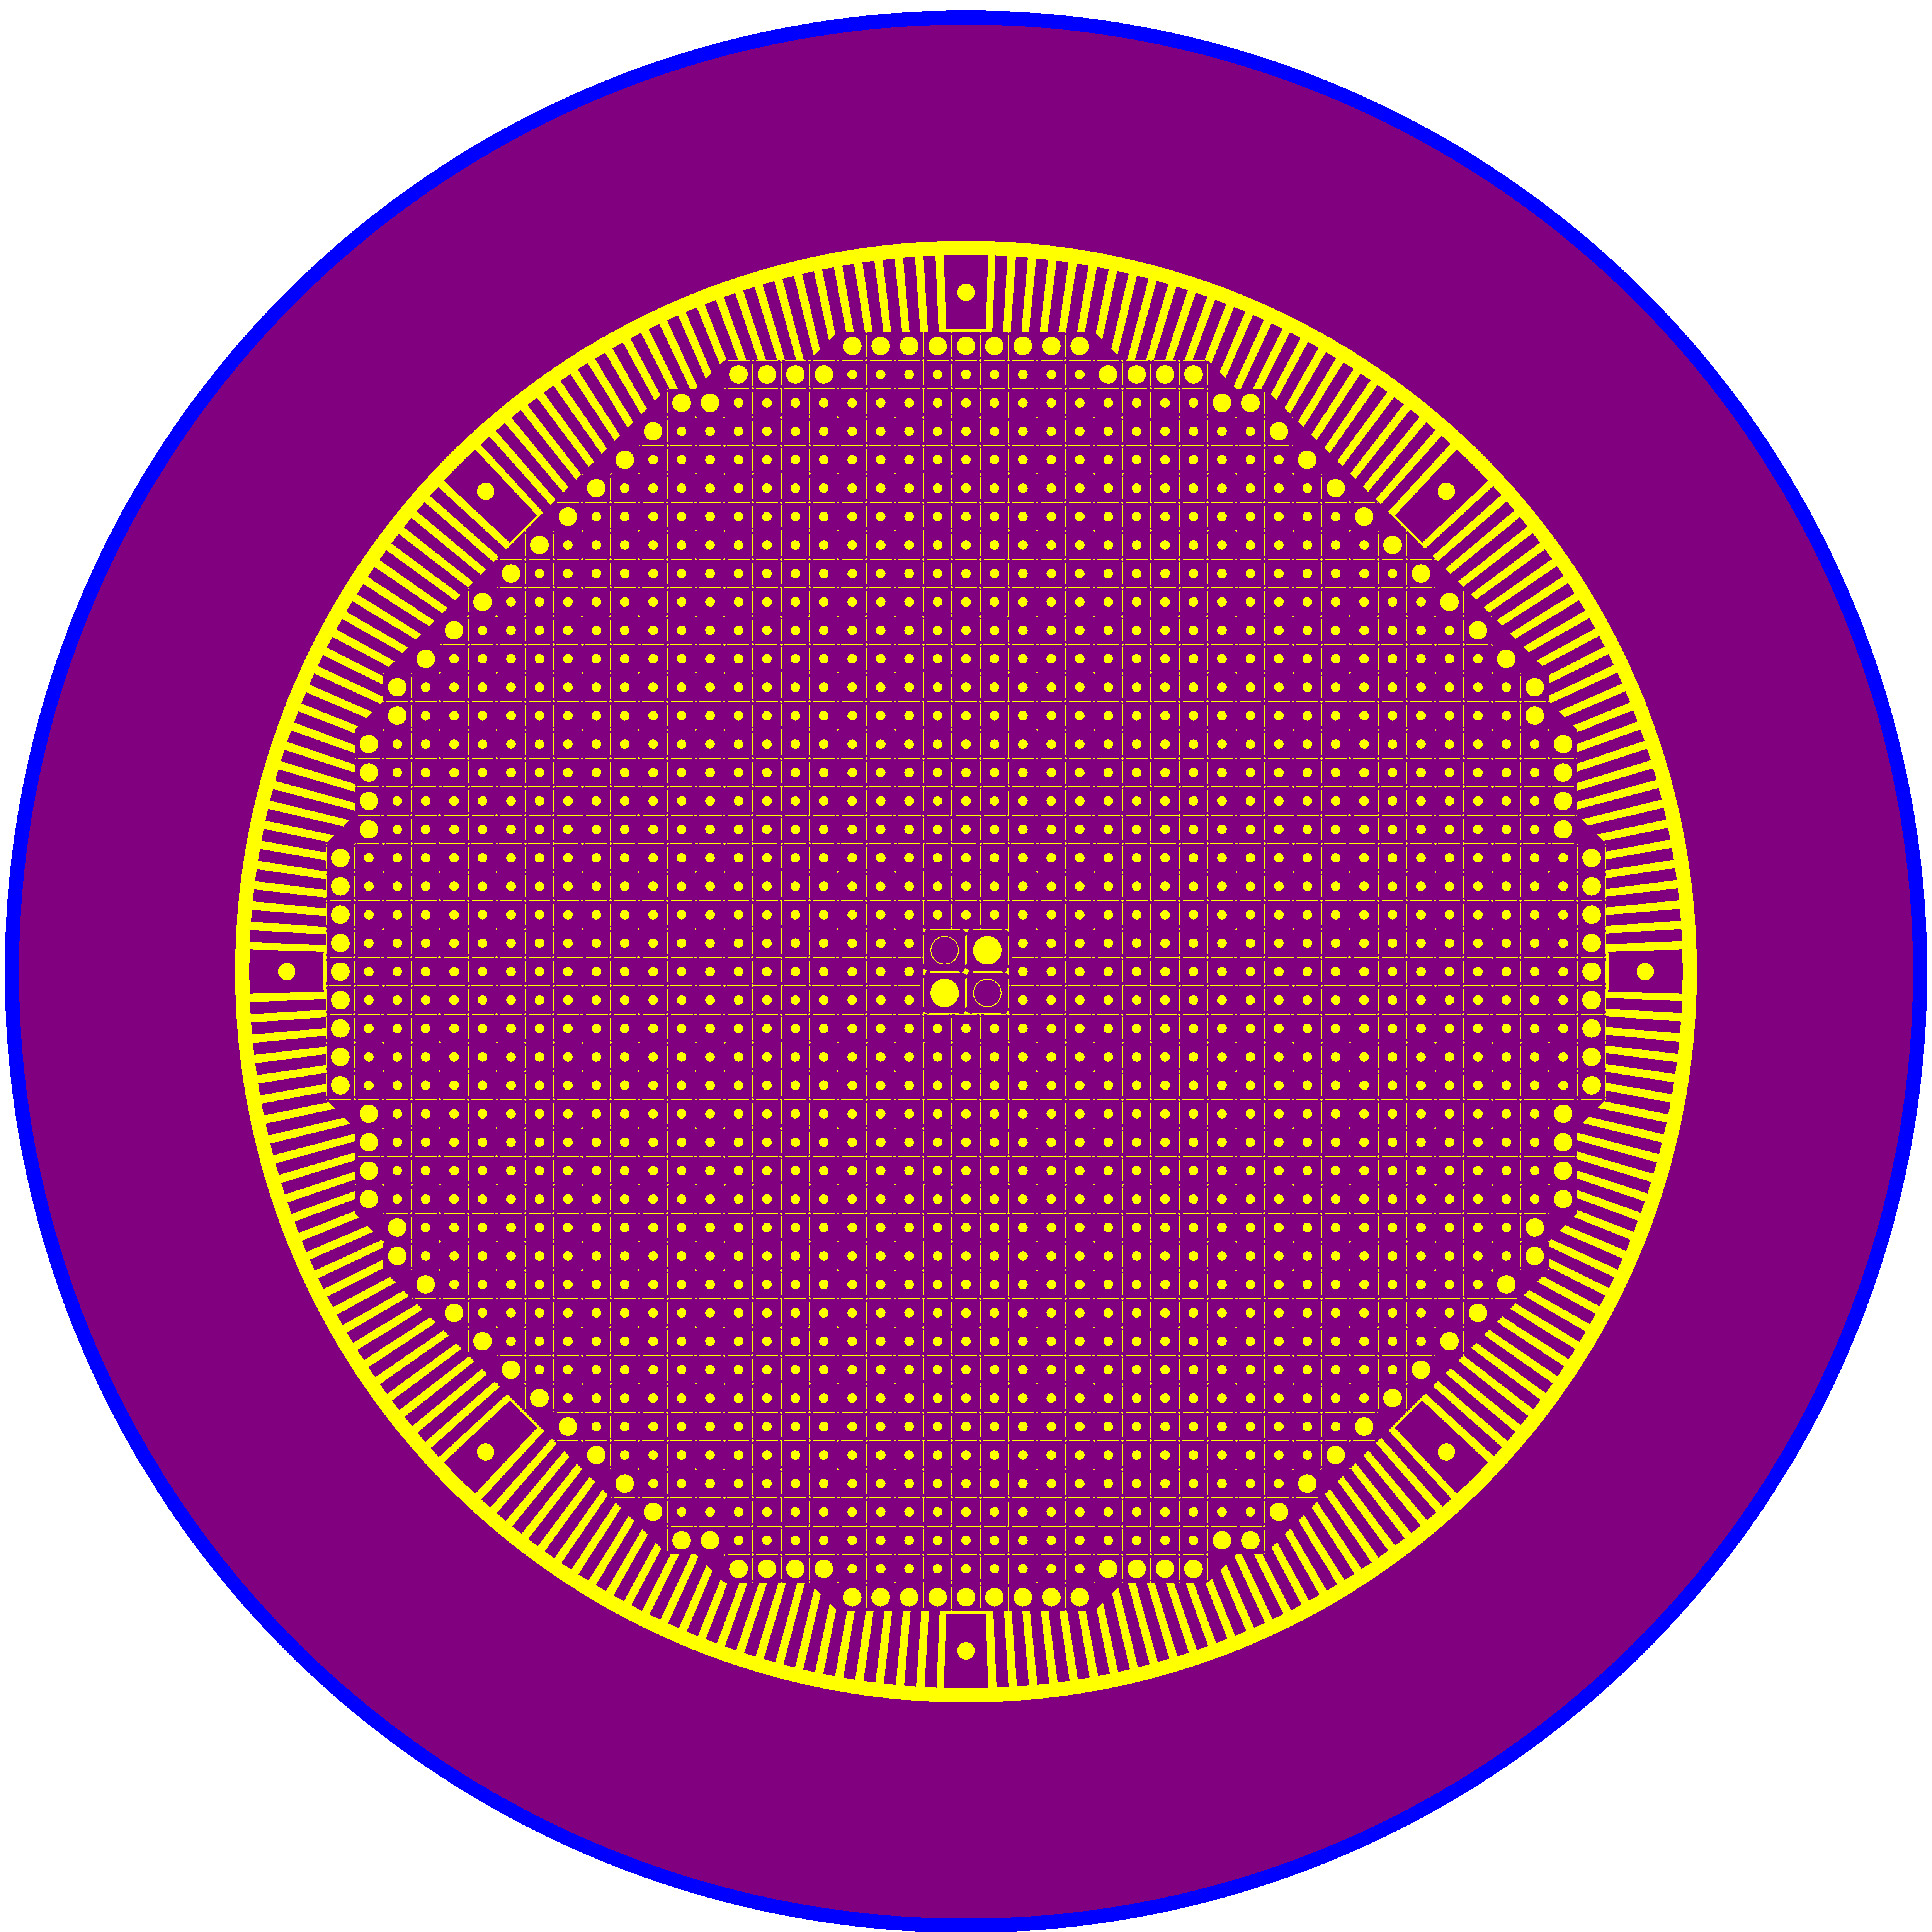
\includegraphics[width=0.5\linewidth]{figs/ch4/msbr_full_xy_openmc.png}
        \label{fig:msbr_model_xy}
    }
    \\
    \subfloat[][]{
        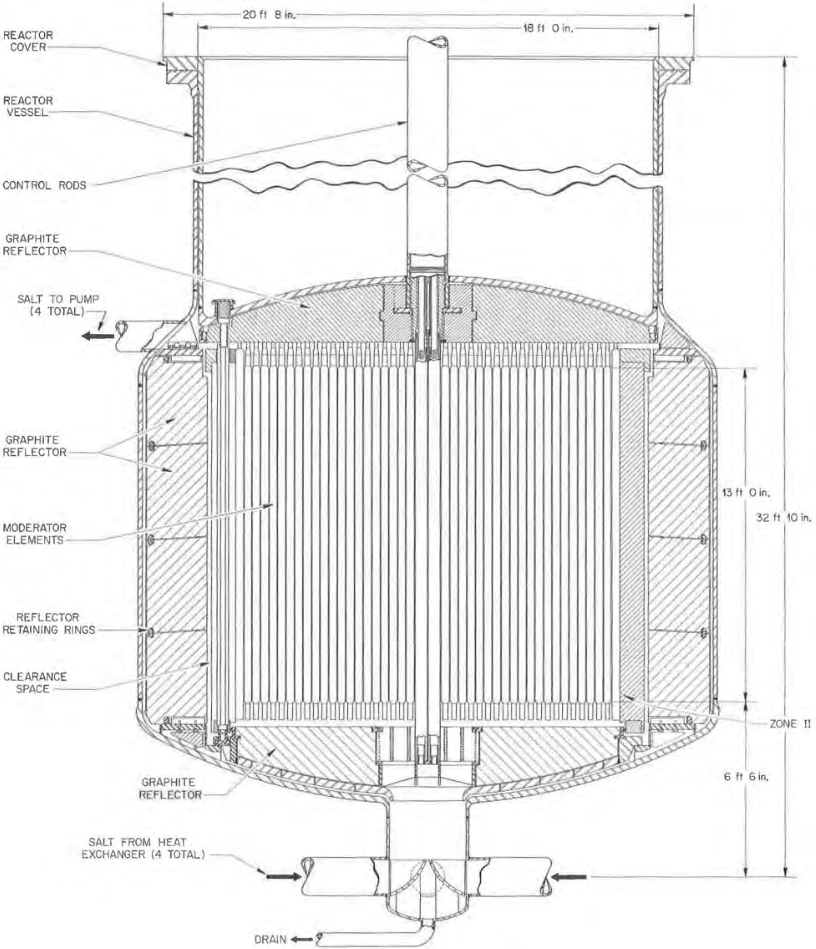
\includegraphics[width=0.5\linewidth]{figs/ch4/msbr_full_xz_ref.png}
        \label{fig:msbr_ref_xz}
    }
    \subfloat[][]{
        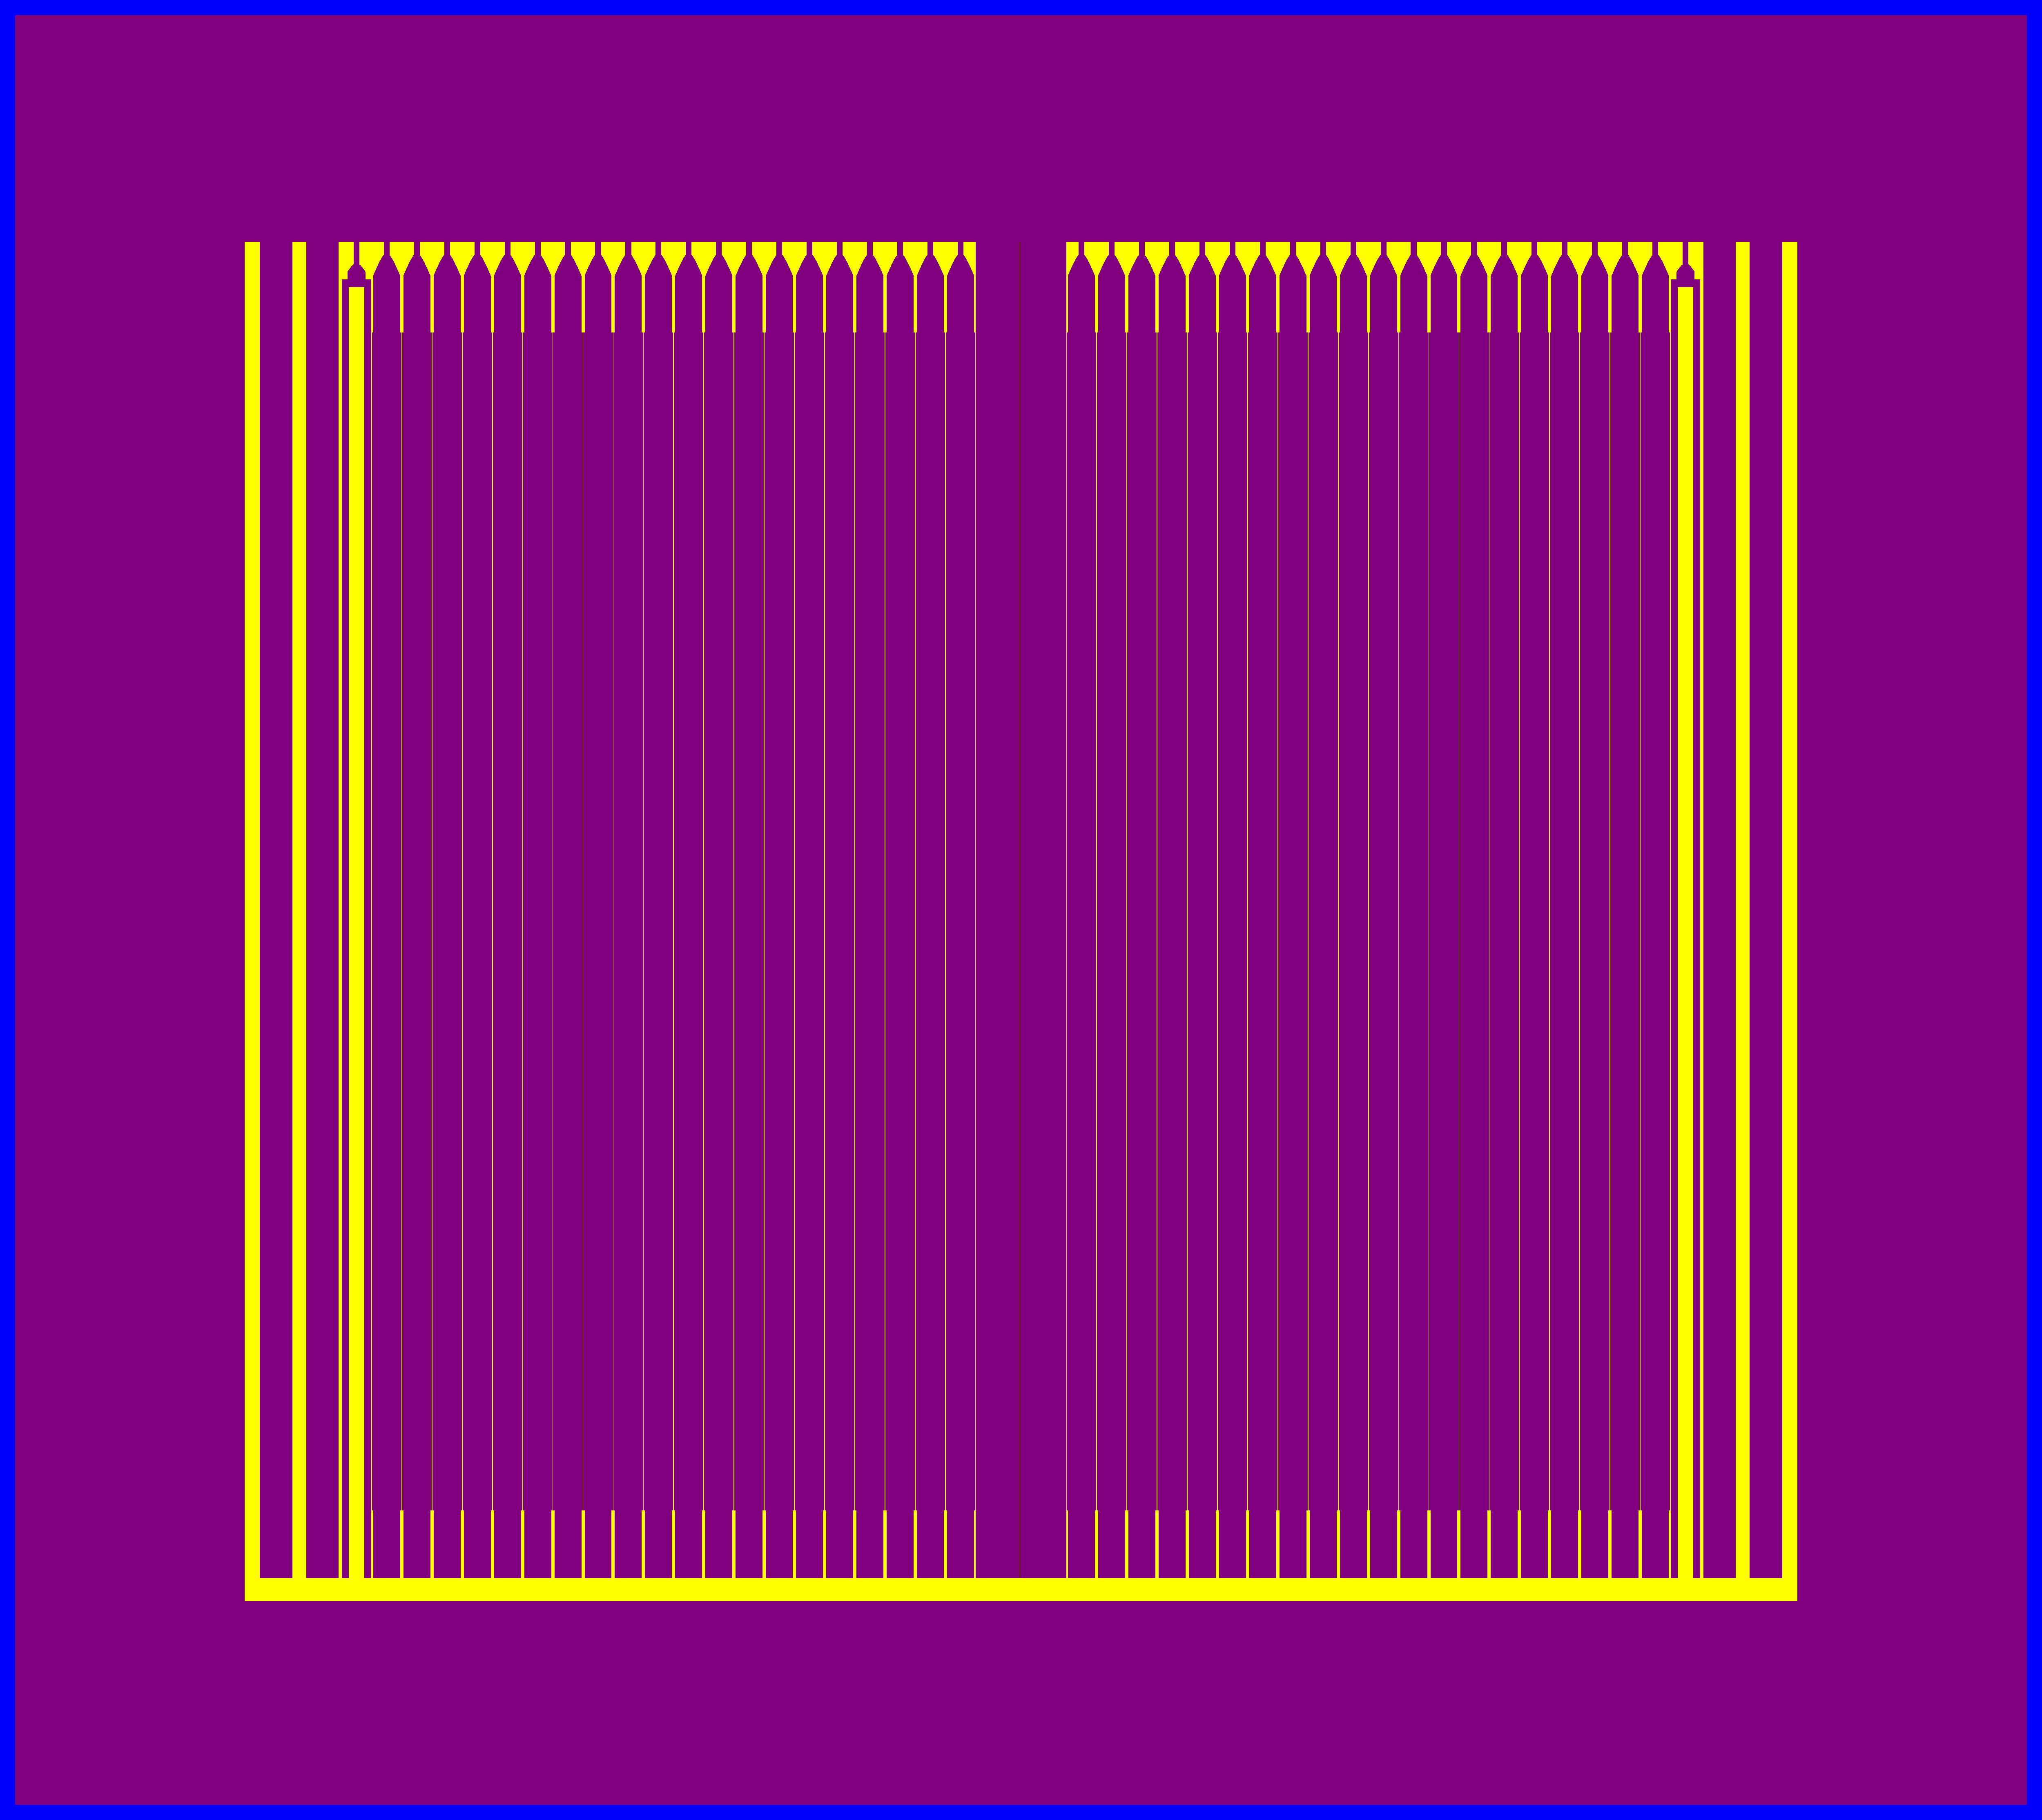
\includegraphics[width=0.5\linewidth]{figs/ch4/msbr_full_xz_openmc.png}
        \label{fig:msbr_model_xz}
    }
    \caption[Full core views of MSBR reference design and virtual model]{
        \subref{fig:msbr_ref_xy} Top down view of \Gls{msbr} reference design.
        \subref{fig:msbr_model_xy} Top down view of \Gls{msbr} CSG model.
        \subref{fig:msbr_ref_xz} Top down view of \Gls{msbr} reference design.
        \subref{fig:msbr_model_xz} Top down view of \Gls{msbr} CSG model.
    }
\end{figure}

As seen in Figure \ref{fig:msbr-overview} \OpenMC and \SerpentTWO \Gls{msbr}
models of reproduce these systems with several approixmations. I will
describe each reactor system, as well as any relavant changes or
approximations made in the model.

\section{Materials}
\label{sec:msbr-materials}

\subsection{Fuel salt}
\label{sub:msbr-fuel-salt}
Table S.1 in \cite{robertson_conceptual_1971} specifies the fuel salt
composition used in the \Gls{msbr}:
\ce{LiF}-\ce{Be}\ce{F_2}-\ce{Th}\ce{F_4}-\ce{U}\ce{F_4} at a
concentration of 71.7-16-12-0.3 mole-\%\footnote{In Rykhlevskii's thesis
\cite{rykhlevskii_fuel_2020}, he stated the mole-\% to be 71.75-16-12-0.25. I
have been unable to find this composition in Robertson et al.
\cite{robertson_conceptual_1971}}. The lithium used in the fuel salt is
enriched to 99.995\% \ce{^{7}Li}. This is because \ce{^{6}Li} is a strong
neutron absorber and produces tritium in the absorption reaction. The atom-\%
for each nuclide is given in Table \ref{tab:msbr_fuel_salt-ref}\footnote{Most of the
discussion of the fuel salt compositon in Robertson el al
\cite{robertson_conceptual_1971} specify elemental version of the nuclides in
Table \ref{tab:msbr_fuel_salt-ref}. I have specific specific nuclides for the
following reasons: (1) both \ce{F} and \ce{Be} have only one stable isotope, (2)
the fuel salt recieves initial fissile loading from \ce{^{233}U} or
\ce{^{235}U}, and (3) the fuel salt recieves its fertile loading from
\ce{^{232}Th}}.

\begin{table}[htpb] 
    \centering 
    \caption{Reference \Gls{msbr} fuel salt specifications}
    \label{tab:msbr_fuel_salt-ref}
    \begin{tabular}{|c|c|c|c|c|c|c|} 
        \hline
        & \ce{^{6}Li} & \ce{^{7}Li} & \ce{^{19}F} & \ce{^{9}Be} & \ce{^{232}Th} & \ce{^{233}U}\\
        \hline 
        atom-\% & 1.4357925 & 34.4142075 & 56.35$\overline{6}$ & 5.$\overline{3}$ & 2.4 & 0.06 \\
        \hline
        mass-\% & 0.4452449 & 12.4477343 & 55.1982285 & 2.4779439 & 28.7100003 & 0.7208481\\ 
        \hline
    \end{tabular}
\end{table}

The density of the fuel salt is given by a function\footnote{This function 
comes from an earlier report on the Molten-Salt Reactor Program
\cite{rosenthal_molten-salt-ornl_1970}.} of temperature in \unit{\celsius} in Table
S.1 in Robertson et al. \cite{robertson_conceptual_1971}:
\begin{equation}
    \rho = 3.752 - 6.68\cdot 10^{-4} \cdot T \quad \unit{\gram\per\square  \centi\meter}
\end{equation}

The temperature of the fuel salt flowing into the core at the inlet at the
bottom of the reactor is 1050\unit{\degree}F (565.5556\unit{\celsius}, 838.7056
\unit{\kelvin}), and the temperature of the fuel salt flowing out of the core at
the outlet is approximately 1300\unit{\degree}F (704.4444\unit{\celsius},
977.5944 \unit{\kelvin})\cite{robertson_conceptual_1971}. The average
temperature of the salt over the core inlets and outlets is then 1175
\unit{\degree}F (635\unit{\celsius}, 908.15 \unit{\kelvin}). While the
various solid components of the core are at a slightly higer temperature on
average\footnote{see figure 3.29 in \cite{robertson_conceptual_1971}}, for
simplicity, I set the evaluated temperature of all materials to 900
\unit{\kelvin} consistent cross-section selection between the \OpenMC and
\SerpentTWO depletion steps. At this temperature, the density of the fuel salt
is 3.3332642 \unit{\gram\per\centi\metre\cubed}.

\begin{table}[htpb] 
    \centering 
    \caption{Model \Gls{msbr} fuel salt specifications}
    \label{tab:msbr_fuel_salt-model}
    \begin{tabular}{|c|c|c|c|c|c|} 
        \hline
        & \ce{^{7}Li} & \ce{^{19}F} & \ce{^{9}Be} & \ce{^{232}Th} & \ce{^{233}U}\\
        \hline 
        atom-\% & 28.386326 & 60.437153 & 6.330058 & 4.747557 & 0.098907 \\
        \hline
        mass-\% & 7.87474673879085 & 45.4003012179284 & 2.25566879138321 & 43.5579130482336 & 0.911370203663893\\ 
        \hline
    \end{tabular}
\end{table}
In the virtual model, the fuel salt material uses the composition specified in
Table \ref{tab:msbr_fuel_salt-model} and has a density of 3.35
\unit{\gram\per\centi\metre\cubed}. Notice that the lithium has been enriched to
100\% \ce{^{7}Li}. This is because during inital simulations, even those very
small amounts of \ce{^{6}Li} were enough to kill the reaction. The inital
fissile and fertile loading has also been slightly increased.

\subsection{Graphite}
\label{sub:graphite}

For a detailed description of the reactor graphite used in the \Gls{msbr}, see
Section 3.2.3 in \cite{robertson_conceptual_1971}. At 70\unit{\degree}F (294.3
\unit{\kelvin}), the \Gls{msbr} graphite has a density of 1843
\unit{\kilo\gram\per\cubic\metre}. This is the only density specification
for graphite that I was able to find in Robertson et al.
\cite{robertson_conceptual_1971}

In the virtual model, the graphite material uses elemental carbon and has a
density of 1.84\unit{\gram\per\centi\metre\cubed}.

\subsection{Modified Hastelloy N}
\label{sub:hastelloy}
Hastelloy N is an alloy developed at \Gls{ornl} during the Molten-Salt Reactor
Program as a structural material that could maintain structural stability while
in contact with the corrosive and high temperature molten salt fuel while also
being under irradation for a long period of time.

The \Gls{msbr} used a modified version of Hastelloy N designed to improve
embrittlement resistance and weldibility \cite{robertson_conceptual_1971}.
The \Gls{msbr} uses modified Hastelloy N on all nearly all salt-facing
components included in the virtual model.

Modified Hastelloy N has a density of 8671 \unit{\kilo\gram\per\cubic\metre} at
1300\unit{\degree}F (704.4444\unit{\celsius}, 977.5944 \unit{\kelvin})
\cite{robertson_conceptual_1971}. The elemental composition of modified
Hastelloy N and their amounts in mass-\% are in Table \ref{tab:hastelloy-n-ref}.

\begin{table}[htpb]
    \centering
    \caption{Mass-\% of elements in modified Hastelloy N used in the \Gls{msbr}. Data from Table 3.1 and S.1 in \cite{robertson_conceptual_1971}. Ranged values collapsed to their average are denoted with a $^*$}
    \label{tab:hastelloy-n-ref}
    \begin{tabular}{|c|c|c|c|c|c|c|c|c|c|c|c|c|c|c|c|c|}
        \hline
        \ce{Ni} & \ce{Mo}$^*$ & \ce{Cr}$^*$ & \ce{Fe}$^*$ & \ce{C}$^*$ & \ce{Mn}$^*$ & \ce{Si} & \ce{W} & \ce{Al} & \ce{Ti}$^*$ & \ce{Cu} & \ce{Co} & \ce{P} & \ce{S} & \ce{B} & \ce{Hf}$^*$ & \ce{Nb}$^*$ \\
        \hline
        73.709 & 12 & 7 & 3 & 0.06 & 0.35 & 0.1 & 0.1 & 0.1 & 1.25 & 0.1 & 0.2 & 0.015 & 0.015 & 0.001 & 1 & 1\\
        %\hline
        %atom-\% & 76.72 & 7.64 & 8.224 & 3.282 & 0.305 & 0.389 & 0.218 & 0.033 & 0.226 & 1.595 & 0.096 & 0.207 & 0.03 & 0.029 & 0.006 & 0.342 & 0.658 \\
        \hline
    \end{tabular}
\end{table}

\begin{table}[htpb]
    \centering
    \caption{Mass-\% of elements in modified Hastelloy N used in the \Gls{msbr} model.}
    \label{tab:hastelloy-n-model}
    \begin{tabular}{|c|c|c|c|}
        \hline
        \ce{Ni} & \ce{Cr} & \ce{W} & \ce{Al} \\
        \hline
        67.7 & 7.0 & 25.0 & 0.3 \\
        \hline
    \end{tabular}
\end{table}

The Hastelloy N material in the virtual model uses the composition specified in
Table \ref{tab:hastelloy-n-model} and has a density of 8.671 
\unit{\gram\per\centi\metre\cubed}. The model material has a different composition
than the reference material because\ldots


\section{Reactor core}
\label{sec:msbr-core}
The \Gls{msbr} core is split into three distinct different zones; zone I, zone
II, and the reflector zone.

\subsection{Zone I} Zone I is the central-most region of the core, and is 13\%
fuel salt by volume. Zone I is divided into three subzones: zone I-A, zone I-B,
and the control rod zone. (more about these zones)

\subsection{Zone II}


\subsection{Reflectors}

\section{Vessel}
\label{sec:msbr-vessel}

\section{Reprocessing system}
\label{sec:msbr-reprocessing-system}

\section{Cross Section Data}

\section{Summary}
